% Adapted from Alex Reustle's CMSC351 Course Notes

% This program is free software: you can redistribute it and/or modify
% it under the terms of the GNU General Public License as published by
% the Free Software Foundation, either version 3 of the License, or
% (at your option) any later version.

% This program is distributed in the hope that it will be useful,
% but WITHOUT ANY WARRANTY; without even the implied warranty of
% MERCHANTABILITY or FITNESS FOR A PARTICULAR PURPOSE.  See the
% GNU General Public License for more details.

% You should have received a copy of the GNU General Public License
% along with this program.  If not, see <http://www.gnu.org/licenses/>.
\documentclass[english, 10pt]{article}

\usepackage{notes}
\usepackage{inconsolata}
\usepackage[shellescape]{gmp}
\allowdisplaybreaks%
\newcommand{\thiscoursecode}{CMSC 216}
\newcommand{\thiscoursename}{Introduction to Computer Systems}
\newcommand{\thisprof}{Dr.\ Ilchul Yoon}
\newcommand{\me}{Akilesh Praveen}
\newcommand{\thisterm}{Spring 2020}
\newcommand{\website}{http://cs.umd.edu/class/spring2020/cmsc216/}%chktex 8
\usepackage{ifpdf}
\ifpdf%
\DeclareGraphicsRule{*}{mps}{*}{}
\fi
% \listfiles

\usepackage[utf8]{inputenc}
 
\usepackage{listings}
\usepackage{xcolor}
 
\definecolor{codegreen}{rgb}{0,0.6,0}
\definecolor{codegray}{rgb}{0.5,0.5,0.5}
\definecolor{codepurple}{rgb}{0.58,0,0.82}
\definecolor{backcolour}{rgb}{0.95,0.95,0.94}
\definecolor{codered}{rgb}{0.5,0.15,0.15}
\definecolor{commentred}{rgb}{1,0.01,0.02}
 
\lstdefinestyle{mystyle}{
    backgroundcolor=\color{backcolour},   
    commentstyle=\color{codegreen},
    keywordstyle=\color{red},
    numberstyle=\tiny\color{codegray},
    stringstyle=\color{codered},
    basicstyle=\ttfamily\footnotesize,
    breakatwhitespace=false,         
    breaklines=true,                 
    captionpos=b,                    
    keepspaces=true,
    xleftmargin=.15\textwidth,
    xrightmargin=.15\textwidth,
    linewidth=\textwidth,                 
    numbers=left,                    
    numbersep=5pt,                  
    showspaces=false,                
    showstringspaces=false,
    showtabs=false,                  
    tabsize=2,
    belowskip=3em,
    aboveskip=3em,
}

\lstset{style=mystyle}


% \VerbEnvir{align tikzpicture algorithm}
%%%Headers
\chead{216-Introduction to Computer Systems}
\lhead{\thisterm}

%%%%% TITLE %%%%%
\graphicspath{{../}}
\newcommand{\notefront}{%
\pagenumbering{arabic}
\begin{center}
{\small}
\textbf{\Huge{\noun{\thiscoursecode}}}
{\Huge \par}
{\Large{\noun{\thiscoursename}}}\\
\vspace{0.1in}
\vspace{0in}
\includegraphics[scale=0.3]{umd_cs.jpg} \\
\vspace{0.1in}{\noun\me} \\
{\noun\thisprof} \ $\bullet$ \ {\noun\thisterm} \ $\bullet$ \ {\noun{University of Maryland}} \\
{\ttfamily \url{\website}} \\
\end{center}
}

 \tikzstyle{class}=[
    rectangle,
    draw=black,
    text centered,
    anchor=north,
    text=black,
    text width=2cm,
    shading=axis,
    bottom color={rgb:red,222;green,222;blue,222},
    top color=white,shading angle=45]

\begin{document}
% \renewcommand\familydefault{\sfdefault}
% \sffamily
  % Notes front
  \notefront%
  % Table of Contents and List of Figures
  \tocandfigures%
  
\section{Notes \& Preface}

This is a compilation of my notes for CMSC216 as a TA for the Spring 2020 offering of the course at the University of Maryland. All content covered in these notes was created by Dr. Ilchul Yoon and Dr. A.U. Shankar at the University of Maryland.
\newline

The actual content of this note repository is the content that I cover as a TA during my discussion section, combined with my personal insights for the course. I took this course with Nelson Padua-Perez in the Spring 2019 offering, so some of the notes that I'll drop in here are from my own notes when I took the course in 2019. As such, I would like to attribute certain code examples, analogies, and more to Mr. Perez. I believe that together, these will serve as great \textbf{supplementary material} for CMSC216, but I would still highly recommend attending all of your lecture and discussion sections to achieve success in CMSC216.
\newline

The notes template in use is Alex Reustle's template, which can be found on his github at the following location: \texttt{https://github.com/Areustle/CMSC351SP2016FLN}
\linebreak

I maintain this repository and as such, take responsibility for any mistakes. Please send errors to \texttt{apraveen@cs.umd.edu}
  
  
\section{Week 1 - Introduction to CMSC216}

CMSC216 is where you learn how a computer works on a much lower level than you've experienced before. There are 3 main components that the course will explore.

\subsection{Overview}

\begin{itemize}
	\item \textbf{UNIX} Threads, processes, and pipes as the building blocks of much bigger applications. We will be working with the UNIX operating system on the development environment at \texttt{grace.umd.edu}
	\item \textbf{C} is a high-performance language that works at a much lower level than Java. Things like memory management and advanced data structures are left up to the user. We'll cover concepts like memory management, pointers, and system calls.
	\item \textbf{Assembly} is even lower-level than C, and studying it will reveal how processors process instructions, store data, and maintain a stack and a heap. It's the lowest level you'll go in this class. For this semester's 216, you will be using MIPS assembly.
\end{itemize}

\subsection{Grace}

In this class, we will be using the \texttt{Grace} system to do all of our work. It's a little confusing to understand at first, so here's my way of thinking about it. In CMSC132, we did all of our work on our own computers. We pulled the skeleton code for the projects from the 132 website/repository, edited the code on our computers, and then uploaded our code to the submit server (via Eclipse) in order to test it.\newline

In CMSC216, we have been given access to this big computer that UMD CS owns known as \texttt{Grace}. You, as a student, have been given a small chunk of that machine to call your own (for the semester). In this class, we will access your files on the \texttt{Grace} system using a program known as \texttt{ssh} (that's how MobaXTerm works) and do all of our editing + running code on \texttt{Grace} itself. In fact, we will also be submitting our projects from \texttt{Grace} to the UMD CS submit server.\newline

Here are the relevant links for getting it all set up. You'll need to setup  \texttt{Grace} and \texttt{gcc} (the C compiler that we'll be using within \texttt{Grace}).\newline\newline
\begin{itemize}
	\item \texttt{\href{http://www.cs.umd.edu/~nelson/classes/resources/GraceSystem.shtml}{http://www.cs.umd.edu/~nelson/classes/resources/GraceSystem.shtml}}
	\item \texttt{\href{http://www.cs.umd.edu/~nelson/classes/resources/setting_gcc_alias.shtml}{http://www.cs.umd.edu/~nelson/classes/resources/setting\_gcc\_alias.shtml}} 
\end{itemize}
 



\subsection{Useful UNIX Commands}

Although the UNIX environment may seem confusing at first, learning it is essential to navigating the Grace environment. Below are some of the basic commands that you may find useful when getting started.

\begin{itemize}
	\item \textbf{\texttt{ssh}} $\rightarrow$ If you are not using MobaXTerm, you will have to access grace using the \texttt{ssh} command. For the purpose of logging in for CMSC216, I recommend adding the \texttt{-y} flag in order to bypass the warning it will give you. E.g. \texttt{ssh -y yourdirectoryid@grace.umd.edu}
	\item \textbf{\texttt{ls}} $\rightarrow$ The \texttt{ls} command lists all the files in your current directory. You can use the \texttt{-l} flag to get more detailed information. E.g. \texttt{ls}, \texttt{ls -l}
	\item \textbf{\texttt{cd}} $\rightarrow$ The \texttt{cd} command changes the directory you're currently in, mainly to directories that you can see with \texttt{ls}. Typing \texttt{cd ..} will navigate one directory 'up' from your current directory, and \texttt{cd} without anything else will return you to your home directory. E.g. \texttt{cd 216public}
	\item \textbf{\texttt{pwd}} $\rightarrow$ This command displays your current directory. Useful for finding out where exactly you are in the UNIX file hierarchy. E.g. \texttt{pwd}
	\item \textbf{\texttt{cp}} $\rightarrow$ Copies files. If you use the \texttt{-r} flag, you're telling the command to recursively copy. If you want to use \texttt{cp} on directories, remember to use that flag.
	\item \textbf{\texttt{rm}} $\rightarrow$ This command stands for 'remove'. It can be used to remove singular files, or can alternatively be used with the \texttt{-r} flag to recursively remove directories. E.g. \texttt{rm hello.c}, \texttt{rm -r project1} (project1 would be a folder.
	\item \textbf{\texttt{.}}, \textbf{\texttt{..}}, \textbf{\texttt{~}}, and \textbf{\texttt{/}} $\rightarrow$ These abbreviations are pretty important. They can be used to navigate a filesystem in Unix and generate some clever commands. In order, they mean 'current directory', 'parent directory', 'user home folder', and 'root directory'. Below are some examples.
	\begin{itemize}
		\item \textbf{\texttt{cp *.c ../}} $\rightarrow$ Copies all files that end with \texttt{.c} to the parent directory.
		\item \textbf{\texttt{cd /}} $\rightarrow$ Changes directories to the root directory.
		\item \textbf{\texttt{cp -r ~/216public/projects/project1 .}} $\rightarrow$ Recursively copies (this means that it copies directories as well as files) the project1 directory and everything in it into the current directory.
	\end{itemize}
\end{itemize}

Lots of these UNIX commands are super useful once you get to know them, but it may be hard becoming acquainted with how they work from the outset. It's a far cry from the GUI you had in CMSC132, so here are a few tips.

\begin{itemize}
	\item If you're just starting out and still need a graphical representation of the filesystem, I'd highly recommend setting up \textbf{MobaXTerm}. The program provides just a little more graphical representation than just a pure terminal, and allows you to navigate the Grace filesystem more freely. I like to think of it as training wheels as you get acquainted with Grace.
	\item I'd highly recommend getting used to making folders, deleting folders, deleting files, and navigating up and down through the filesystem with rapid sequences of \texttt{ls} and \texttt{cd}. As with all things, practice makes perfect, and pretty soon you'll be a command line wizard.
\end{itemize}

\subsection{Machine}

A computer is composed of several parts, but a great way to think about it is a few main components connected by a \textbf{bus}. \newline

\begin{itemize}
	\item \textbf{Memory} can just be thought of as a contiguous array of bytes. At the end of the day, this is the stuff that has to be written to/read from.
	\item \textbf{I/O Devices} are connected to the CPU via a bus, like mentioned above. By performing read/write operations to the right adaptor, the CPU is able to interface with different I/O devices.
	\item \textbf{CPU} is the central processing unit of the computer. It handles computational operations (arithmetic, logic, etc.) and interfaces with the memory and I/O devices via the bus. The CPU is also responsible for performing the \textbf{fetch-execute cycle}.
\end{itemize}

A bus is like one main connector that's responsible for making sure the CPU, memory, and I/O devices are all able to interface with each other.\newline\newline
Note that in this course, we won't be going too in-depth into hardware (that's more Computer Engineering), but it's great background knowledge to have as you approach this class, which is why I have included it here.

\section{Week 2}

\subsection{The Math Library}

We won't be using the math library much in C, but for the times that we do, just remember this one simple flag that we add to the gcc command. As an example, if you try to write some code that includes the math library like below, you'll find that it won't compile with a regular \texttt{gcc} command. 

{\centering
\begin{lstlisting}[language=C]
#include <stdio.h>
#include <math.h>

int main() {
   double value;

   printf("Enter a number: ");
   scanf("%lf", &value);     /* Notice the use of %lf */

   printf("sqrt %f: \n", sqrt(value));
   printf("power of 2: %f\n", pow(value, 2));
   printf("sin: %f\n", sin(value));

   return 0;
}
\end{lstlisting}
}

In this class we won't be using libraries that require this specific compilation option too much, but remember that the \texttt{-lm} flag essentially enables us to use the math library.

\subsection{Using Emacs}

Most of the instruction for this course will be done in \texttt{emacs}, a highly versatile text editor that you can use in GUI form or from the command line. It's always an option to use other text editors in this class, but I would recommend using \texttt{emacs}, as it's what all the in-class demos are in. There is a way to setup IDEs like Visual Studio Code to function with Grace, but I won't cover them here. I believe that although graphical IDEs have their advantages, you'll get plenty of experience with them in CMSC330 and CMSC4XX, so for now, develop your skills in a command line editor like \texttt{emacs} or \texttt{vi}.\newline

For your benefit, here are some basic commands in \texttt{emacs} that I've found useful over the time that I took 216.\newline\newline
\textbf{Note:} When I indicate to type \texttt{M}, that means you need to press the 'meta' key. On most machines, the 'meta' key is the 'alt/option'. When I indicate to type \texttt{C}, I mean the 'control' key. The reason I'm using this notation is because it's the same notation that online guides use to describe \texttt{emacs} shortcuts.

\begin{itemize}
	\item \textbf{\texttt{C-x C-s}} $\rightarrow$ Saves the file you're working on. Remember to do this frequently on Grace, as you can't guarantee that your connection to Grace will stay intact.
	\item \textbf{\texttt{C-x C-c}} $\rightarrow$ Closes the file that you're working on. If you haven't saved, it will prompt you to save.
	\item \textbf{\texttt{C-x u}} $\rightarrow$ Undo the previous command that you ran.
	\item \textbf{\texttt{C-s}} $\rightarrow$ Search forwards (this will search for text that'll be ahead of where your cursor is now.)
	\item \textbf{\texttt{C-r}} $\rightarrow$ Search backwards (this will search for text that'll be behind where your cursor is now.)
	\item \textbf{\texttt{C-l}} $\rightarrow$ This command will center the window around your cursor. A great technique when you have large C files that you're editing.
	\item \textbf{\texttt{M-x column-number-mode}} $\rightarrow$ Shows column numbers. Useful if you want to check if you're above the 80 character limit.
\end{itemize}

\subsection{Debugging}

There are three main debugging tools that we use in 216: Valgrind, GDB, and splint. For now, we won't focus too much on Valgrind, as it's more oriented towards helping programmers get rid of memory leaks and other memory-related issues. We will focus on GDB and Splint.

\subsubsection{GDB}

GDB Is the C equivalent of the Eclipse Debugger. It lets you do everything that the Eclipse Debugger allowed you to do in CMSC131 and CMSC132. The only real drawback here is that it's all done from the command line, so the graphic part of the interface is a little lacking. However, it's an essential tool that I'd highly recommend using to figure out errors in your code.\newline

Online references will tell you that there are a lot of commands that you need to know to effectively use GDB, but here are some of the ones that I've found useful.

\begin{itemize}
	\item \textbf{\texttt{q}} $\rightarrow$ exits gdb. Useful.
	\item \textbf{\texttt{start}} $\rightarrow$ starts running your code with a temporary breakpoint at the first line of main(). This allows you to set more breakpoints before the code actually starts executing.
	\item \textbf{\texttt{l}} $\rightarrow$ lists the code that you have.
	\item \textbf{\texttt{b}} $\rightarrow$ typing p with a number next to it sets a breakpoint at a line. E.g. \texttt{b 3}
	\item \textbf{\texttt{n}} $\rightarrow$ the equivalent of step over in the Eclipse debugger
	\item \textbf{\texttt{s}} $\rightarrow$ the equivalent of step into in the Eclipse debugger
	\item \textbf{\texttt{c}} $\rightarrow$ will continue running your code until the next breakpoint
	\item \textbf{\texttt{p}} $\rightarrow$ will print the value of an expression or a variable. E.g. \texttt{p valid\_character('x')}.
\end{itemize}

In order to start GDB, you'll first need to compile your C code into an \texttt{a.out} file. Not only that, but I would recommend that you compile your code with the \texttt{-ggdb} flag, to ensure that GDB initializes your program correctly. In order to run GDB with your newly compiled program, remember to just type \texttt{gdb a.out}\newline 

\section{Week 3}

This week we go over a lot of general C-specific programming concepts in discussion, and that material is heavier than what we usually do in discussion. In that sense, I'll try and go over the more basic stuff that I think will be highly useful as you work on your projects.

\subsection{Comma is an Operator}

The comma in C is an operator. The best way to think about this in use is when you're declaring multiple variables at once, like when you say \texttt{int i, j = 2}.

Remember, commas are \textbf{also} used as separators in C. A great example would be if you're giving a function multiple parameters, like in \texttt{printf("\%d and \%d", i, j)}. When you consider the comma as an operator in C, it's always important to understand where it's an operator vs. where it's a separator. 

Although we don't think about the comma operator quite a lot, one of the main reasons for understanding it would be initialization of multiple variables in a loop. Take a look at the following example from my notes (from a previous offering of the CMSC216 course).

{\centering
\begin{lstlisting}[language=C]
// Comma Operator Example by Nelson Padua-Perez

for (j=0, k=10; j<=limit; j++, k+= 10) {
	printf("j->%d, k->%d\n", j, k);
} 
\end{lstlisting}
}

Notice how you initialize and increment multiple variables within a single for-loop.


\subsection{Identifier Scope}

Scope exists in C in a similar way that it does in other languages. All you have to remember is that if you declare variables within code blocks, they won't be accessible outside those blocks. In that regard, this phenomenon is quite similar to how Java handles scopes.

\subsection{C Program Memory Organization}

As we delve deeper into systems-level programming, it's important to visualize how C actaully manages the memory that your programs use. The interesting part about this is that this diagram is an exact representation of system memory, so you're finally able to see 'under the hood' of your programs.\newline

You can see that the lowest address is represented by \texttt{0x0} and the highest address is represented by \texttt{0xffffffff}. These addresses are actual locations in memory, represented in hexadecimal format (hence ffffffff being the highest address in the representation).

\begin{center}

\tikzset{every picture/.style={line width=0.75pt}} %set default line width to 0.75pt        

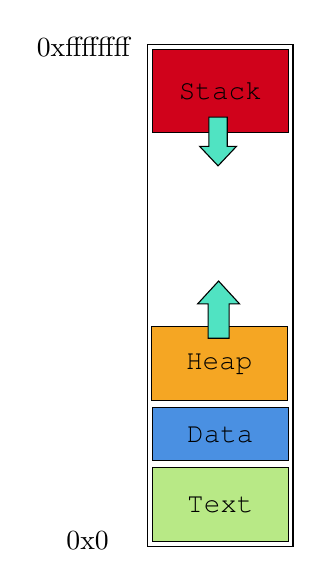
\begin{tikzpicture}[x=0.75pt,y=0.75pt,yscale=-1,xscale=1]
%uncomment if require: \path (0,300); %set diagram left start at 0, and has height of 300

%Shape: Rectangle [id:dp1982436807499255] 
\draw   (330,23) -- (400,23) -- (400,265) -- (330,265) -- cycle ;
%Shape: Rectangle [id:dp02798297576071851] 
\draw  [fill={rgb, 255:red, 184; green, 233; blue, 134 }  ,fill opacity=1 ] (332.25,227) -- (397.75,227) -- (397.75,262.5) -- (332.25,262.5) -- cycle ;
%Shape: Rectangle [id:dp8690208046922276] 
\draw  [fill={rgb, 255:red, 74; green, 144; blue, 226 }  ,fill opacity=1 ] (332.25,197.83) -- (397.75,197.83) -- (397.75,223.33) -- (332.25,223.33) -- cycle ;
%Shape: Rectangle [id:dp6529311675516911] 
\draw  [fill={rgb, 255:red, 245; green, 166; blue, 35 }  ,fill opacity=1 ] (331.75,158.83) -- (397.25,158.83) -- (397.25,194.58) -- (331.75,194.58) -- cycle ;
%Up Arrow [id:dp9371264302671377] 
\draw  [fill={rgb, 255:red, 80; green, 227; blue, 194 }  ,fill opacity=1 ] (354,148.03) -- (364.13,137) -- (374.25,148.03) -- (369.19,148.03) -- (369.19,164.58) -- (359.06,164.58) -- (359.06,148.03) -- cycle ;
%Shape: Rectangle [id:dp8515554275840291] 
\draw  [fill={rgb, 255:red, 208; green, 2; blue, 27 }  ,fill opacity=1 ] (332.25,25.5) -- (397.75,25.5) -- (397.75,65.5) -- (332.25,65.5) -- cycle ;
%Down Arrow [id:dp38470823955499234] 
\draw  [fill={rgb, 255:red, 80; green, 227; blue, 194 }  ,fill opacity=1 ] (355,72.1) -- (359.44,72.1) -- (359.44,58) -- (368.31,58) -- (368.31,72.1) -- (372.75,72.1) -- (363.88,81.5) -- cycle ;

% Text Node
\draw (365,211.25) node   [align=left] {{\fontfamily{pcr}\selectfont Data}};
% Text Node
\draw (365,244.75) node   [align=left] {{\fontfamily{pcr}\selectfont Text}};
% Text Node
\draw (364.5,176.71) node   [align=left] {{\fontfamily{pcr}\selectfont Heap}};
% Text Node
\draw (365,45.5) node   [align=left] {{\fontfamily{pcr}\selectfont Stack}};
% Text Node
\draw (299,24) node   [align=left] {0xffffffff};
% Text Node
\draw (301,262) node   [align=left] {0x0};



\end{tikzpicture}

\end{center}


Your program is allocated a certain block of memory- within it are the following 4 components. Keep in mind that this too, is an abstraction. You can further explore how programs are represented in memory in classes like CMSC411, but this is just about as far as we'll go in 216.

\begin{itemize}
	\item \textbf{Text} is where the code for your program goes. It's really not much more complex than that.
	\item \textbf{Data} is where global variables and variables that are static belong.
	\item \textbf{Heap} is where dynamically allocated memory lives. In Java, this stuff was managed for you. In C, you will have to manage it yourself, allocating memory and effectively increasing the size of the heap if you need more space while your program is running, and deallocating (freeing) memory to decrease the size of the heap. More on this when we discuss dynamically allocated memory.
	\item \textbf{Stack} is where local variables and function parameters live. It grows downwards (eventually meeting the heap and causing a stackoverflow) as functions are called. If you'll think back to 'stack frames' from recursion in CMSC132, this is the exact same concept.
\end{itemize}

\subsection{Storage}

There are two types of ways variables are stored in C- automatic and static. This basically goes hand-in-hand with block scopes and file scopes, but the important takeaways are these. First of all, in the example below, after the function \texttt{foo} is called, the variable \texttt{n} is thrown away.

{\centering
\begin{lstlisting}[language=C]
int foo(int k) {
	int n = 216;
	return n;
}
\end{lstlisting}
}

In that regard, the variable \texttt{n} has automatic storage. If a variable has static storage, it basically exists throughout the duration of your program's running time. Such variables are initialized only once.\newline

An important note: \texttt{static} in C does not mean the same thing as it does in Java. Here are the two main things that I think are worth remembering about static variables in C:

\begin{itemize}
	\item Static variables need not necessarily be initialized. If you don't bother initializing a static variable (you still have to declare it- this is not Python, language of the heathen) it will automatically initialize to zero.
	\item Static variables retain their values between function invocations. In other words, they are not stored using automatic storage.
\end{itemize}

{\centering
\begin{lstlisting}[language=C]
// example from Nelson Padua-Perez

void compute_static(int x) {                                                    
   static int value = 100; /* What would happen if we don't initialize it? */         
                                                                                
   printf("(static) x: %d, value: %d, sum: %d \n", x, value, value + x);        
                                                                                
   ++value;                                                                     
} 
\end{lstlisting}
}

In the example above, if you called \texttt{compute\_static} twice, then your output would be \texttt{(static) x: 1, value: 100, sum: 101} and \texttt{(static) x: 1, value: 101, sum: 102}, as 'value' would retain its data between function calls.

\subsection{Linkage}

Linkage is essentially the science behind having C code spread across multiple files and making sure it all compiles and works properly.\newline

We want to sometimes split code between multiple files for organizational purposes. Currently, the projects you're working on are small, but in order to make your programs versatile, modular and better organized, it's a great idea to split code between files.\newline

When you attempt this, there may be issues that follow. For example, you may encounter a situation where you want to name a function \texttt{print\_sum()} in two files. How would we deal with such a duplicate?\newline

Problems of this sort can be solved by adjusting the \textbf{linkage} of these functions.\newline

For actual code examples, please check the linkage-examples in the 216public directory. They're extremely thorough. My goal here is to provide a quick few tips on what I think are the most important parts.\newline

Essentially, there are three types of linkage that you should remember to guide you through writing code in multiple C files.

\begin{itemize}
	\item \textbf{\texttt{None}} $\rightarrow$ No linkage. This is how you usually declare your variables, and as you'd expect, doesn't do anything special in regards to linkage. Think of it this way: A variable with no linkage belongs to a single function, and cannot be shared. In other words, there is \textit{only one copy per declaration}.
	\item \textbf{\texttt{Internal}} $\rightarrow$ Internal linkage is just a fancy way of saying you're using the \textbf{\texttt{static}} keyword. All declarations of a single identifier in file refer to the same thing. In other words, there is \textit{only one copy per file}.
	\item \textbf{\texttt{External}} $\rightarrow$ External linkage is signified by the \texttt{extern} identifier, and it basically means that a name can only refer to a single entity in your entire program. In other words, there is \textit{only one copy per program}.
\end{itemize}

\subsection{Enumerated Types}

Enumerated Types, or enums, in C are pretty useful, and quite comparable to their equivalents in Java. The best way to understand enums (in my opinion) is to think of examples. Some good ones are an enum for the days of the week (Monday, Tuesday, etc.), seasons (Summer, Spring, Fall, Winter), or even suits in a deck of cards (Spades, Clubs, Hearts, Diamonds). Below is an example of the latter.

{\centering
\begin{lstlisting}[language=C]
// example from Nelson Padua-Perez
#include <stdio.h>
int main() {
	enum Suit {SPADES, HEARTS,DIAMONDS = 42, CLUBS};
	enum Suit suit1, suit2;
	suit1 = SPADES;
	suit2 = CLUBS;
	if (suit1 < suit2) printf("Spades are first.\n");
	else printf("Clubs are first.\n");
	printf("Spades = %d, Clubs = %d\n",suit1, suit2);
	return 0;
}
\end{lstlisting}
}

The functionality here is pretty basic, but one thing that I think is worth remembering (and quite nifty if you can use it well) is that enum representations are based in integers. This means that, for example, you can get away with adding the month enum for January (0) and the month enum for February (1) and end up with February (1).\newline

Again, the code above is a great example of how you can leverage the integer-like characteristics of enums.

\subsection{Implicit Type Conversion and Casting in C}

Switching between data types is pretty similar to how it was in Java, but here's a quick review of the stuff that matters. As you write your projects, you'll realize these things, but it's important to remember when it's a good idea to cast and when it isn't. Here are some general tips for you.\newline

\begin{itemize}
	\item \texttt{int}s are the smallest data type. If you need to describe something as a number and want to be as efficient as possible without getting fancy, the good old integer is the best way to go.
	\item We can also cast in C, and it works almost the same was as it did in Java. Just remember, in Java we had the concept of wrapper classes that allowed us to do fancy things with certain data types. In C, we don't enjoy that luxury, so we are restricted to just basic data type casting. Below is an example.
	
	
	{\centering
\begin{lstlisting}[language=C]
// example from Nelson Padua-Perez

#include <stdio.h>                                                                    
                                                                                      
int main() {                                                                          
   float x = 2.98;
   int y = (int)x;
}
\end{lstlisting}
}

\item That works exactly as you think it does. It converts 2.98 to 2 as it would in Java. Remember, don't overthink it, and don't try to call any wrapper class methods that you remember from Java. As long as you keep that in mind, you should be good to convert between data types in C.
\end{itemize}

	{\centering
\begin{lstlisting}[language=C]
// example from Nelson Padua-Perez

#include <stdio.h>                                                                    
                                                                                      
int main() {                                                                          
   int x = 2000000000;                                                                
   long result_long;                                                                  
                                                                                      
   printf("Value of x: %d\n", x);                                                     
   printf("Multiplying by 3 (with %%d format): %d\n", 2000000000 * 3);                
   printf("Multiplying by 3 (with %%ld format): %ld\n", 2000000000 * 3);              
   printf("Multiplying by 3L (with %%d format): %d\n", 2000000000 * 3L);              
   printf("Multiplying by 3L (with %%ld format): %ld\n", 2000000000 * 3L);            
                                                                                      
   result_long = 2000000000 * 3;  /* Does it solve the problem? */                    
   printf("Storing result in long type variable: %ld\n", result_long);                
                                                                                      
   return 0;                                                                          
}
\end{lstlisting}
}

The above example from Nelson isn't that basic, but I feel like it gives you a good insight into how type conversion can find use. Give that example a try to see a cool application of using multiple data types to handle larger values. 


\section{Closing Thoughts}

This document will be updated frequently as we progress through CMSC216. Please send errors to \texttt{apraveen@cs.umd.edu}

\end{document}